\documentclass[,%fontsize=11pt,%
			paper=a4,% 
			%DIV12, % mehr text pro seite als defaultyyp
			DIV14,
			%DIV=calc,%
			%twoside=false,%
			liststotoc,
			bibtotoc,
			draft=false,% final|draft % draft ist platzsparender (kein code, bilder..)
			%titlepage,
			numbers=noendperiod
			]{scrartcl}


\usepackage[utf8]{inputenc}
\usepackage[T1]{fontenc}
\usepackage[english]{babel}


%\usepackage{vaucanson-g}
%\usepackage{amssymb}
%\usepackage{latexsym}

% for color-highlighted code
%\usepackage{color} % for grey comments
%\usepackage{alltt}

%\usepackage[doublespacing]{setspace}
\usepackage[onehalfspacing]{setspace}
%\usepackage[singlespacing]{setspace}
\usepackage{tabularx}
%\usepackage{hyperref}
\usepackage{comment}
\usepackage{color}
\usepackage{url}      % for urls
\usepackage{multicol}
\usepackage{float}
\usepackage{caption}
\usepackage{amsmath}
\usepackage{mathtools}
\usepackage{amssymb}

\usepackage{soul}

\newcommand{\mst}{\textbf{MST}}
\newcommand{\kmst}{\textit{k}-\mst}

\definecolor{grey2}{gray}{.90}
\sethlcolor{grey2}
\newcommand{\ilc}[1]{\hl{\texttt{#1}}} % ilc = inline code

\title{Report on the implementation of the \kmst\ problem as integer linear program}
\author{Bernhard Mallinger \\ 0707663 \and Christof Schmidt \\ 0627958}

\begin{document}

\maketitle

\section{Problem description}

The \kmst\ problem is a variation of the Minimum Spanning Tree (\mst) problem for undirected graphs $G = (V, E, w)$, including a weight function $w(e) : E \rightarrow \mathbb{R}^+_0$.
The goal of both problems is to find a tree of minimum cost, but instead of requiring it to span the whole graph as in the classical \mst, for the \kmst, the tree has to span a given number of $k$ arbitrary nodes.
This restriction turns the formerly tractable problem into an $NP$-complete one.

\section{General formulation}

This section describes all variables and constraints, that the formulations for connectivity share. It deals mostly with representing the graph as well as ensuring acyclicity.

In order to represent the graph, we chose to use a Boolean array \ilc{edges} containing a directed variants of the originally undirected edges.
This will simplify the management of flow later on.
\ilc{edges} contains $2|E|$ elements, where the first half represents the edges in one direction and the other half the opposite ones.
Since trees are acyclic, we can require that only one of the two directed edges that are derived from an undirected edge in the original graph are chosen:
\begin{equation}
 \ilc{edges}[i] + \ilc{edges}[i + |E|] \leq 1\quad\forall~0\leq i \leq |E|
\end{equation}

Furthermore, to avoid circles in the set of solutions, we require that each vertex has at most one incoming edge (\eqref{eq:oneIncoming}) with a special treatment of the artificial root node, which must not have any incoming edge at all (\eqref{eq:root0}) but exactly one outgoing node (\eqref{eq:root1}). 
As the connectivity constraints take effect later, this will ensure that once a node is reached from the root node, there cannot be a path back it (which would form a circle), since then the number of incoming edges would exceed 1.
In order to add the constraints only for the relevant and existing edges, we implemented two auxiliary functions: \ilc{incomingEdges}, which returns for a node \ilc{j} the set of indices in the \ilc{edges}-array which correspond to edges incoming to \ilc{j}, and \ilc{outgoingEdges}, which works analoguously for outgoing edges.

\begin{equation}\label{eq:oneIncoming}
	\sum_{\mathclap{i\,\in\,\ilc{incomingEdges(j)}}} \ilc{edges}[i] = 1 \quad \forall j \in V
\end{equation}
\begin{equation}\label{eq:root0}
	\sum_{\mathclap{i\,\in\,\ilc{incomingEdges(0)}}} \ilc{edges}[i] = 0
\end{equation}
\begin{equation}\label{eq:root1}
	\sum_{\mathclap{i\,\in\,\ilc{outgoingEdges(0)}}} \ilc{edges}[i] = 1 
\end{equation}

Finally, it is still necessary to state the size of the tree to be calculated.
The problem statement requires the tree to have exactly $k$ nodes, which for trees means that there are $k-1$ edges.
Since this formulation also includes an artificial root node, that is not part of the actual problem, we need to allow a further edge, resulting in $k-1+1=k$ edges in total.
\begin{equation}
	\sum_{i=0}^{2|E|} \ilc{edges}[i] = k
\end{equation}

\section{Connectivity formulations}

The central task of this exercise is to ensure the connectivity of the tree, which can be achieved with any of the following formulations.
The sections are split up into the essential core formulations and strengthening constraints, which are not necessary for correctness but lead to a tighter formulation.

\subsubsection{Strengthening Constraints}
All models were subject to the following constraint, that implies a tighter model. It forces all nodes that do not have an incoming edges to not have any outgoing nodes. Unfortunatly, that does not guarantee connectedness, since it still allows circles.
\begin{equation}\label{eq:StrAll}
	 \sum_{{\forall \ilc{edge} \in \ilc{edges} | \ilc{edge.v2} = \ilc{v}}} \ilc{edge} * k
\geq
 \sum_{{\forall \ilc{edge} \in \ilc{edges} | \ilc{edge.v1} = \ilc{v}}} \ilc{edge} 
\quad \forall \ilc{v} \in V \textbackslash \{0\}
\end{equation}

\subsection{Single Commodity Flow Formulation}

The idea of this formulation is to produce flow at the root node, of which every vertex of the solution consumes one unit.
This consumption however can only take place if the flow is delivered to the node on a path that consists of solution edges.
If such a path from the root node to every solution node exists, it is ensured that these vertices are connected.

The concrete modelling is based upon an array of flow values for each edge named \ilc{flow\_scf}.
The variables of this array are constrained to take nonnegative values up to $k$, where the respective value in \ilc{edges} serves as activation flag: A flow greater than 0 is only allowed in case the edge is taken:
\begin{equation}\label{eq:scf1}
	0 \leq \ilc{flow\_scf}[i] \leq k * \ilc{edges}[i] \quad 0 \leq i \leq 2|E|
\end{equation}

The artificial root node $0$ sends out $k$ units of flow:\nolinebreak
\begin{equation}
	\sum_{\mathclap{i\,\in\,\ilc{outgoingEdges(0)}}} \ilc{flow\_scf}[i] = k
\end{equation}

Flow must be conserved, every vertex of the solution sends out as much as it receives minus the one it consumes. In valid solutions, this constraint is only fulfilled by vertices, that are part of the solution. Those differ from the others by having exactly one incoming edge, which is leveraged as activation flag in this formulation:

\begin{equation}
	\sum_{\mathclap{i\,\in\,\ilc{incomingEdges(j)}}} \ilc{flow\_scf}[i] \quad - \quad
	\sum_{\mathclap{i\,\in\,\ilc{outgoingEdges(j)}}} \ilc{flow\_scf}[i] \quad = \quad 
	\sum_{\mathclap{i\,\in\,\ilc{incomingEdges(j)}}} \ilc{edges\_scf}[i] 
	\quad \forall j\,\in\,V
\end{equation}


\subsubsection{Strengthening constraints}

In \eqref{eq:scf1}, the maximum value for the flow is limited by $k$. However since it's a priori deducible that the first edge can only belong to the set of edges leaving the artificial root node, we can tighten the maximum to $k-1$ for all other nodes, as the source of this edge can at most send out this many units of flow.
\begin{equation}\tag{\ref{eq:scf1}$^\prime$}
	0 \leq \ilc{flow\_scf}[i] \leq k * \ilc{edges}[i] \quad \forall i \in \ilc{outgoingEdges(0)} 
\end{equation}
\begin{equation}\tag{\ref{eq:scf1}$^{\prime\prime}$}
	0 \leq \ilc{flow\_scf}[i] \leq (k-1) * \ilc{edges}[i] \quad \forall i \not\in \ilc{outgoingEdges(0)}
\end{equation}

As further optimisation, we tried to restrict the flow variables to integer values, since in valid solutions, they have to be integer. This turned out to have negative effects on the runtime.


\begin{comment}
	- flow on each edge
	- 0 <= flow\_i <= k/k-1 * edge
	- root note emits
	- every node eats/flow conservation
\end{comment}


\subsection{Multi Commodity Flow Formulation}
The Multi Commodity Flow Formulation is based on the Single Commodity Flow Formulation, but instead of single flow, it defines a flow for each vertex seperatly, called a commodity. Formally the $flow$ is now $\ilc{flow[k][e]} \in \left\{0,1\right\}$ , which is the flow for commodity k, that is destined for vertex k, on the edge $e \in \ilc{edges}$; The flow is send out from the root, forwarded by each node that isn't the destination, and finally consumed by the destination node.

\subsubsection{Additional (re-used) variables}
The \ilc{incomingEdgesSum[commodity]} is defined as the sum of all edges ending in vertex \ilc{commodity} that are part of the \kmst.
\begin{equation}\label{eq:mfcInEdges}
	\ilc{incomingEdgesSum[commodity]} = \sum_{\mathclap{\forall \ilc{edge} \in \ilc{edges} | \ilc{edge.v2} = \ilc{commodity}}} \ilc{edge} 
\quad \forall \ilc{commodity} \in V \textbackslash \{0\}
\end{equation}


\subsubsection{Constraints}

This constraint implies the sending of the commodity for each vertex that is part of the \kmst\ (=has one incoming edge).
\begin{equation}\label{eq:mfcSend}
	\sum_{\mathclap{\forall e|i=0, j \neq 0}}^{} \ilc{flow[commodity][e]} = \ilc{incomingEdgesSum[commodity]}
\quad \forall \ilc{commodity} \in V  \textbackslash \{0\}
\end{equation}

Each vertex recieves his commodity (if part of \kmst).
\begin{equation}\label{eq:mfcRec}
	  \sum_{\mathclap{\forall \ilc{edge} \in \ilc{edges}| \ilc{edge.v2} = \ilc{commodity}}} \ilc{flow[commodity][edge]} 
 = \ilc{incomingEdgesSum[commodity]}
\quad \forall \ilc{commodity} \in V  \textbackslash \{0\}
\end{equation}

Each vertex forwards all other commodities
\begin{equation}\label{eq:mfcForward}
\begin{split}
\sum_{\mathclap i \in \ilc{incomingEdges(v)}} \ilc{flow[commodity][i]} = \sum_{ i \in \ilc{outgoingEdges(v)}} \ilc{flow[commodity][i]} \\
\ \forall ilc{commodity} \in V  \textbackslash \{0\}
\ \forall v \in V  \textbackslash \{0\}
\quad \ilc{commodity} \neq v
\end{split}
\end{equation}

Flow is restricted to selected edges

\begin{equation}\label{eq:mfcFlowEdge}
 \ilc{flow[commodity][e]} \leq \ilc{edges[e]} \quad \forall \forall e \in \ilc{edges}
\forall \ilc{commodity} \in V  \textbackslash \{0\}
\end{equation}

\subsubsection{Strengthening Constraints}

There cannot be flow to the root node.
\begin{equation}\label{eq:mfcNoFlow}
 \ilc{flow[commodity][i]} = 0
\quad \forall i \in \ilc{incomingEdges(0)} | 
\quad \forall \ilc{commodity} \in V
\end{equation}


\subsection{Sequential Formulation}
The sequential formulation, proposed by Miller, Tucker and Zemlin (thus, refered as MTZ) is  based on an additional variable \ilc{u[i]} $\in \{0..u_{max}\}$ for each node i. It gives the tree an order, in which \ilc{u[0]} has the value 0, each node of the \kmst\ has a an increasing value along the path from the root. Nodes, that are not in the \kmst\ get the value $u_{max}$, which is k in our case.

\subsubsection{Constraints}
The main constraint only is active when \ilc{edges[e]} is selected, and thus 1. Otherwise the $u_{max}$ makes sure the constraint always holds. If the edge is selected, it forces the \ilc{u} value of the start of the edge to be at least one less than the end of the edge, this inducing the order.
\begin{equation}\label{eq:mztOrder}
 (\ilc{u[e.start]} + \ilc{edges[e]})  - \ilc{u[e.end]} - ( ( 1 - \ilc{edges[e]}) * u_{max} )  <= 0
\ \ \forall e \in \ilc{edges}
\end{equation}

This constraint forces all u values for unused nodes (which have no incoming nodes) to the value $u_{max}$, so that by above rule \eqref{eq:mztOrder}, that cannot have outgoing edges.
\begin{equation}\label{eq:mztUnused}
 u_{max}*(1 - (\sum_{ i \in \ilc{incomingEdges(v)}} \ilc{edges[i]} )) <= \ilc{u[vertex]}
 \ \forall v \in V  \textbackslash \{0\}
\end{equation}


\subsubsection{Strengthening Constraints}
For all non artificial nodes, we know that the u value has to be at least 1.
\begin{equation}\label{eq:mztNodes1}
 \ilc{u[v]} >= 1
 \ \forall v \in V  \textbackslash \{0\}
\end{equation}

We know that the sum of all u values can be at most $(n-1 - k) * u_{max}$ plus $\sum_1^k{k}$

\begin{equation}\label{eq:mztMaxU}
\sum_{v \in V}{\ilc{u[v]}} \leq u_{max} * ( n - 1 - k ) + {k * (k+1)} / 2
\end{equation}


\section{Results}
We executed all the tests on the provided ADS Server on a single core, without output and in the production compile mode. All but the very large instances have been run several times to minimize the error on the execution times. The last two columns are the results of the formulation without the strengthening constraints.


\subsection{Single Commodity Flow Formulation}

\begin{tabular}{||c||cccr|cr||}

\hline
test     & k & objective  & branch-n-bound & running   & BnB nodes & running\\
instance &   & function   & nodes          & time (sec)& (w/o SC)  & time w/o SC \\
\hline

g01.dat	&	2	&	46	&	0	&	0.012	&	0	&	0.012	\\
g01.dat	&	5	&	477	&	0	&	0.016	&	0	&	0.018	\\
g02.dat	&	4	&	373	&	5	&	0.019	&	5	&	0.019	\\
g02.dat	&	10	&	1390	&	80	&	0.056	&	80	&	0.098	\\
g03.dat	&	10	&	725	&	36	&	0.145	&	36	&	0.098	\\
g03.dat	&	25	&	3074	&	62	&	0.236	&	62	&	0.234	\\
g04.dat	&	14	&	909	&	216	&	0.483	&	216	&	0.353	\\
g04.dat	&	35	&	3292	&	69	&	0.478	&	69	&	0.459	\\
g05.dat	&	20	&	1235	&	119	&	0.447	&	119	&	0.415	\\
g05.dat	&	50	&	4898	&	286	&	1.125	&	286	&	0.934	\\
g06.dat	&	40	&	2068	&	1799	&	11.069	&	1799	&	11.498	\\
g06.dat	&	100	&	6705	&	1587	&	11.215	&	1587	&	11.510	\\
g07.dat	&	60	&	1335	&	282	&	19.275	&	282	&	18.390	\\
g07.dat	&	150	&	4534	&	977	&	48.275	&	977	&	49.095	\\
g08.dat	&	80	&	1620	&	461	&	73.010	&	461	&	70.590	\\
g08.dat	&	200	&	5787	&	461	&	161.705	&	461	&	144.505	\\

\hline

\end{tabular}

\subsection{Multi Commodity Flow Formulation}

\begin{tabular}{||c||cccr|cr||}
\hline
test     & k & objective  & branch-n-bound & running   & BnB nodes & running\\
instance &   & function   & nodes          & time (sec)& (w/o SC)  & time w/o SC \\
\hline

g01.dat	&	2	&	46	&	0	&	0.073	&	0	&	0.074	\\
g01.dat	&	5	&	477	&	0	&	0.054	&	0	&	0.073	\\
g02.dat	&	4	&	373	&	9	&	0.224	&	9	&	0.306	\\
g02.dat	&	10	&	1390	&	0	&	0.212	&	0	&	0.227	\\
g03.dat	&	10	&	725	&	0	&	1.848	&	0	&	1.985	\\
g03.dat	&	25	&	3074	&	0	&	2.383	&	0	&	2.411	\\
g04.dat	&	14	&	909	&	67	&	11.294	&	67	&	10.264	\\
g04.dat	&	35	&	3292	&	0	&	12.378	&	0	&	12.610	\\
g05.dat	&	20	&	1235	&	3	&	37.684	&	3	&	37.666	\\
g05.dat	&	50	&	4898	&	0	&	31.528	&	0	&	31.894	\\
g06.dat	&	40	&	2068	&	231	&	2,180.080	&	231	&	2,134.190	\\
g06.dat	&	100	&	6705	&	9	&	2,016.450	&	9	&	1,996.000	\\
g07.dat	&	60	&	-	&	-	&	-	&	-	&	-	\\
g07.dat	&	150	&	-	&	-	&	-	&	-	&	-	\\
g08.dat	&	80	&	-	&	-	&	-	&	-	&	-	\\
g08.dat	&	200	&	-	&	-	&	-	&	-	&	-	\\

\hline
\end{tabular}


\subsection{Sequential Formulation}

\begin{tabular}{||c||cccr|cr||}
\hline
test     & k & objective  & branch-n-bound & running   & BnB nodes & running\\
instance &   & function   & nodes          & time (sec)& (w/o SC)  & time w/o SC \\
\hline
g01.dat	&	2	&	46	&	0	&	0.006	&	0	&	0.008	\\
g01.dat	&	5	&	477	&	15	&	0.020	&	16	&	0.022	\\
g02.dat	&	4	&	373	&	83	&	0.046	&	102	&	0.040	\\
g02.dat	&	10	&	1390	&	665	&	0.163	&	1039	&	0.185	\\
g03.dat	&	10	&	725	&	601	&	0.344	&	964	&	0.555	\\
g03.dat	&	25	&	3074	&	1494	&	1.822	&	951	&	1.387	\\
g04.dat	&	14	&	909	&	510	&	1.747	&	2879	&	4.444	\\
g04.dat	&	35	&	3292	&	11213	&	20.095	&	17425	&	29.909	\\
g05.dat	&	20	&	1235	&	2362	&	4.695	&	1013	&	2.191	\\
g05.dat	&	50	&	4898	&	12769	&	30.450	&	12735	&	22.332	\\
g06.dat	&	40	&	2068	&	12555	&	117.360	&	26941	&	197.820	\\
g06.dat	&	100	&	6705	&	37379	&	138.460	&	89272	&	331.990	\\
g07.dat	&	60	&	1335	&	68448	&	898.800	&	976440	&	7,869.940	\\
g07.dat	&	150	&	4534	&	22848$^{(*)}$	&	550.99$^{(*)}$	&	-	&	-	\\
g08.dat	&	80	&	-	&	-	&	-	&	-	&	-	\\
g08.dat	&	200	&	5787	&	94744	&	1,601.900	&	258769	&	7,040.260	\\
\hline
\end{tabular}

$^{(*)}$ = Result not from the final model, but a slightly different formulation.

\begin{figure}
	\centering	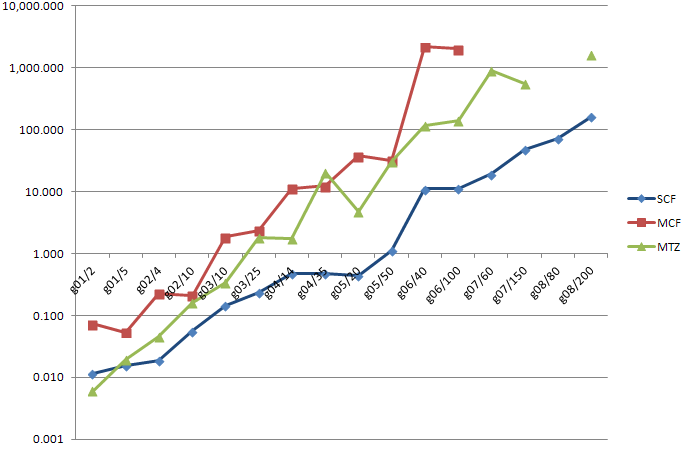
\includegraphics[width=1.00\textwidth]{D:/privat/Algorithmics/algorithmics-prog/report/chart.png}
	\caption{Comparision of runtimes between the models}
	\label{fig:chart}
\end{figure}


\section{Interpretation of results}
Chart ~\ref{fig:chart} shows big differences in the performances of the different formulations. The SCF model performed far better than all other models in most instance sizes and was always albe to compute a result in a reasonable timespan. The MTZ usually yielded better results than the MCF formulation, but for some of the large instances, they were unable to produce results.

...

The MCF wasn't even computable for instances 7 and 8 due to their quadratic number of constraints.

...
We were suprised, that small changes on the model led to very different results, usually the impact was worse for some and better for other instances. In addition, even for the same model and instance, the runtime fluctuated unusually strong. We tried to compensate this effect by executing several rounds of tests. But overall, we cannot rule out chance as the main contributor to the test results, which makes interpreting the results of strengthening a bit of a gamble.

\end{document}
